\documentclass[12pt]{article}

% load packages 
\usepackage{mathptmx}
\usepackage{geometry}
\usepackage{graphicx}
\usepackage{wrapfig}
\usepackage{afterpage}
\usepackage{natbib}
\usepackage{setspace}
\usepackage{abstract}
\usepackage{tocloft}
\usepackage[toc, page, title]{appendix}
\usepackage{multirow}
\usepackage{tabularx}
\usepackage{float}
\usepackage{subcaption}
\usepackage{indentfirst}
\usepackage{sectsty}

% page layout
\geometry{margin=0.8in}
\renewcommand{\arraystretch}{1.5} 
\setlength\parindent{20pt}\setlength{\parskip}{0.0pt plus 0.0pt}

% text formatting
\sectionfont{\large \scshape}
\subsectionfont{\normalsize\itshape}
\subsubsectionfont{\normalsize\mdseries\itshape}
\setcounter{secnumdepth}{3}
\renewcommand{\abstractname}{Résumé}
\setlength{\abstitleskip}{-0.5em}
\renewcommand{\abstractnamefont}{\normalfont \large \bfseries \scshape}
\renewcommand{\abstracttextfont}{\normalfont \normalsize}
\renewcommand\refname{Bibliographie}
\renewcommand{\contentsname}{Sommaire}
\renewcommand{\listfigurename}{Liste des Figures}
\renewcommand{\listtablename}{Liste des Tableaux}
\renewcommand{\appendixtocname}{Annexes}
\renewcommand{\appendixpagename}{\large \scshape \bfseries Annexes}
\renewcommand{\appendixname}{Annexe}
\renewcommand{\setthesection}{\Alph{section}}


% toc formatting
\setlength\cftsecindent{0pt}
\setlength\cftsubsecindent{20pt}
\setlength\cftsubsubsecindent{48pt}
\setlength\cftbeforesecskip{18pt}
\setlength\cftbeforesubsecskip{10pt}
\setlength\cftbeforesubsubsecskip{8pt}
\renewcommand{\cftdot}{.}
\renewcommand{\cfttoctitlefont}{\large \scshape \bfseries}
\renewcommand{\cftloftitlefont}{\large \scshape \bfseries}
\renewcommand{\cftlottitlefont}{\large \scshape \bfseries}
\renewcommand{\cftpnumalign}{l}
\setlength{\cftbeforefigskip}{5pt}
\cftsetpnumwidth{50pt}
\cftsetrmarg{65pt}

% biblio style
\setcitestyle{authoryear,open={(},close={)}}

% figure and table
\floatplacement{figure}{h}
\floatplacement{table}{h}
\setlength\columnsep{20pt}

% empty page
\newcommand\myemptypage{
    \null
    \thispagestyle{empty}
    \addtocounter{page}{-1}
    \newpage
    }


\begin{document}
\begin{titlepage}
\centering
\includegraphics[width=8cm]{img/amu-logo.png}\hfill  \includegraphics[width=4.2cm]{img/logo-ofb.png} \hfill \includegraphics[width=3.7cm]{img/logo-mio.png}\par\vspace{1cm}
{\scshape\large Aix-Marseille Université\par}
{\large Institut OSU-Pythéas\par}
Institut Méditerranéen d’Océanologie - MIO \par
\vspace{2cm}
{\scshape\large Master Sciences de la mer\par}
{\large Parcours Océanographie Biologique et Écologie Marine\par}
\vspace{2cm}
{\LARGE \bfseries Titre du stage\par}
\vspace{.5cm}
{\large \itshape Couteyen Carpaye, Mathilde\par}
\vfill
{\itshape Etude réalisée au sein de l'Institut Méditerranéen d'Océanologie\par}
{\itshape Sous la direction de M. Gérald Grégori et M. David Nérini\par }
\vfill
Année universitaire\par
2021-2022
\end{titlepage}

\myemptypage

\section*{Remerciements}


\newpage


\newpage
\tableofcontents
\newpage


\section{Introduction}


\section{Matériels \& Méthodes}

\subsection{SOMLIT (Service d'Observation en Milieu LITtoral)}

\subsubsection{Les stations}

\subsubsection{Prélèvements et protocoles}

\subsubsection{Jeux de données}

Les données collectées lors des campagnes du SOMLIT sont hébergées dans leur propre base de données.  Les données hydrologiques, biologiques et CTD pour les trois sites d’intérêt, Banyuls, Marseille et Villefranche, ont été téléchargées depuis leur site internet (https://www.somlit.fr/).  Le Tableau 1 résume les données récupérées pour les trois stations. Le jeu de données hydrologiques (HYDRO) contient les données de Température, Salinité, Oxygène, pH, Amonium ($NH_4$), Nitrites ($NO_3$), Nitrates ($NO_2$), Phosphates ($PO_4$), Silice ($Si(OH)_4$) , Carbone Organique Particulaire (COP), Azote Organique Particulaire (NOP) et  Chlorophylle a. Le jeu de données biologiques (PICONANO) contient les données de cytométrie des groupes de plancton présentés précédemment. Pour tous les groupes, on dispose des données d’abondance et de diffusion. Pour le phytoplancton, sont de même disponibles les valeurs d’auto-fluorescence rouge, et pour les bactéries hétérotrophes les valeurs de fluorescence verte. Les valeurs d’auto-fluorescence orange des Synechococcus et des Cryptophytes sont également renseignées. Le jeu de données CTD contient les profils verticaux de la surface au fond pour les variables Température, Salinité, Chlorophylle a et Éclairement. 

Une première visualisation des données brutes permet d’identifier les séries temporelles exploitables et les éventuelles données aberrantes. La Figure 1 présente les données de surface des variables hydrologiques au cours du temps toutes stations confondues. Les éventuelles valeurs aberrantes sont identifiées en rouge. La ligne pointillée orange correspond au début du jeu de données PICONANO et la lignée pointillée bleue correspond à la mise en place du protocole national pour la variable présentée. Étant donné la mise en place tardive d’un protocole standardisé pour le pH, cette variable n’est pas analysée. La mesure de l’Oxygène étant sujette à de nombreux biais liés à la précision de l’échantillonnage, celle-ci est également ignorée. La Figure 2 présente les données de Température de surface et au fond pour les trois stations. Les graphiques nous permettent d’identifier une potentielle inversion des données de fond et de surface à Villefranche entre le début de la série temporelle et 2002. Comme il est impossible de savoir avec certitude quelles observations ont été interverties, les données HYDRO de Villefranche datant d’avant  2002 ne sont pas exploitées. 

\begin{figure}
\centering
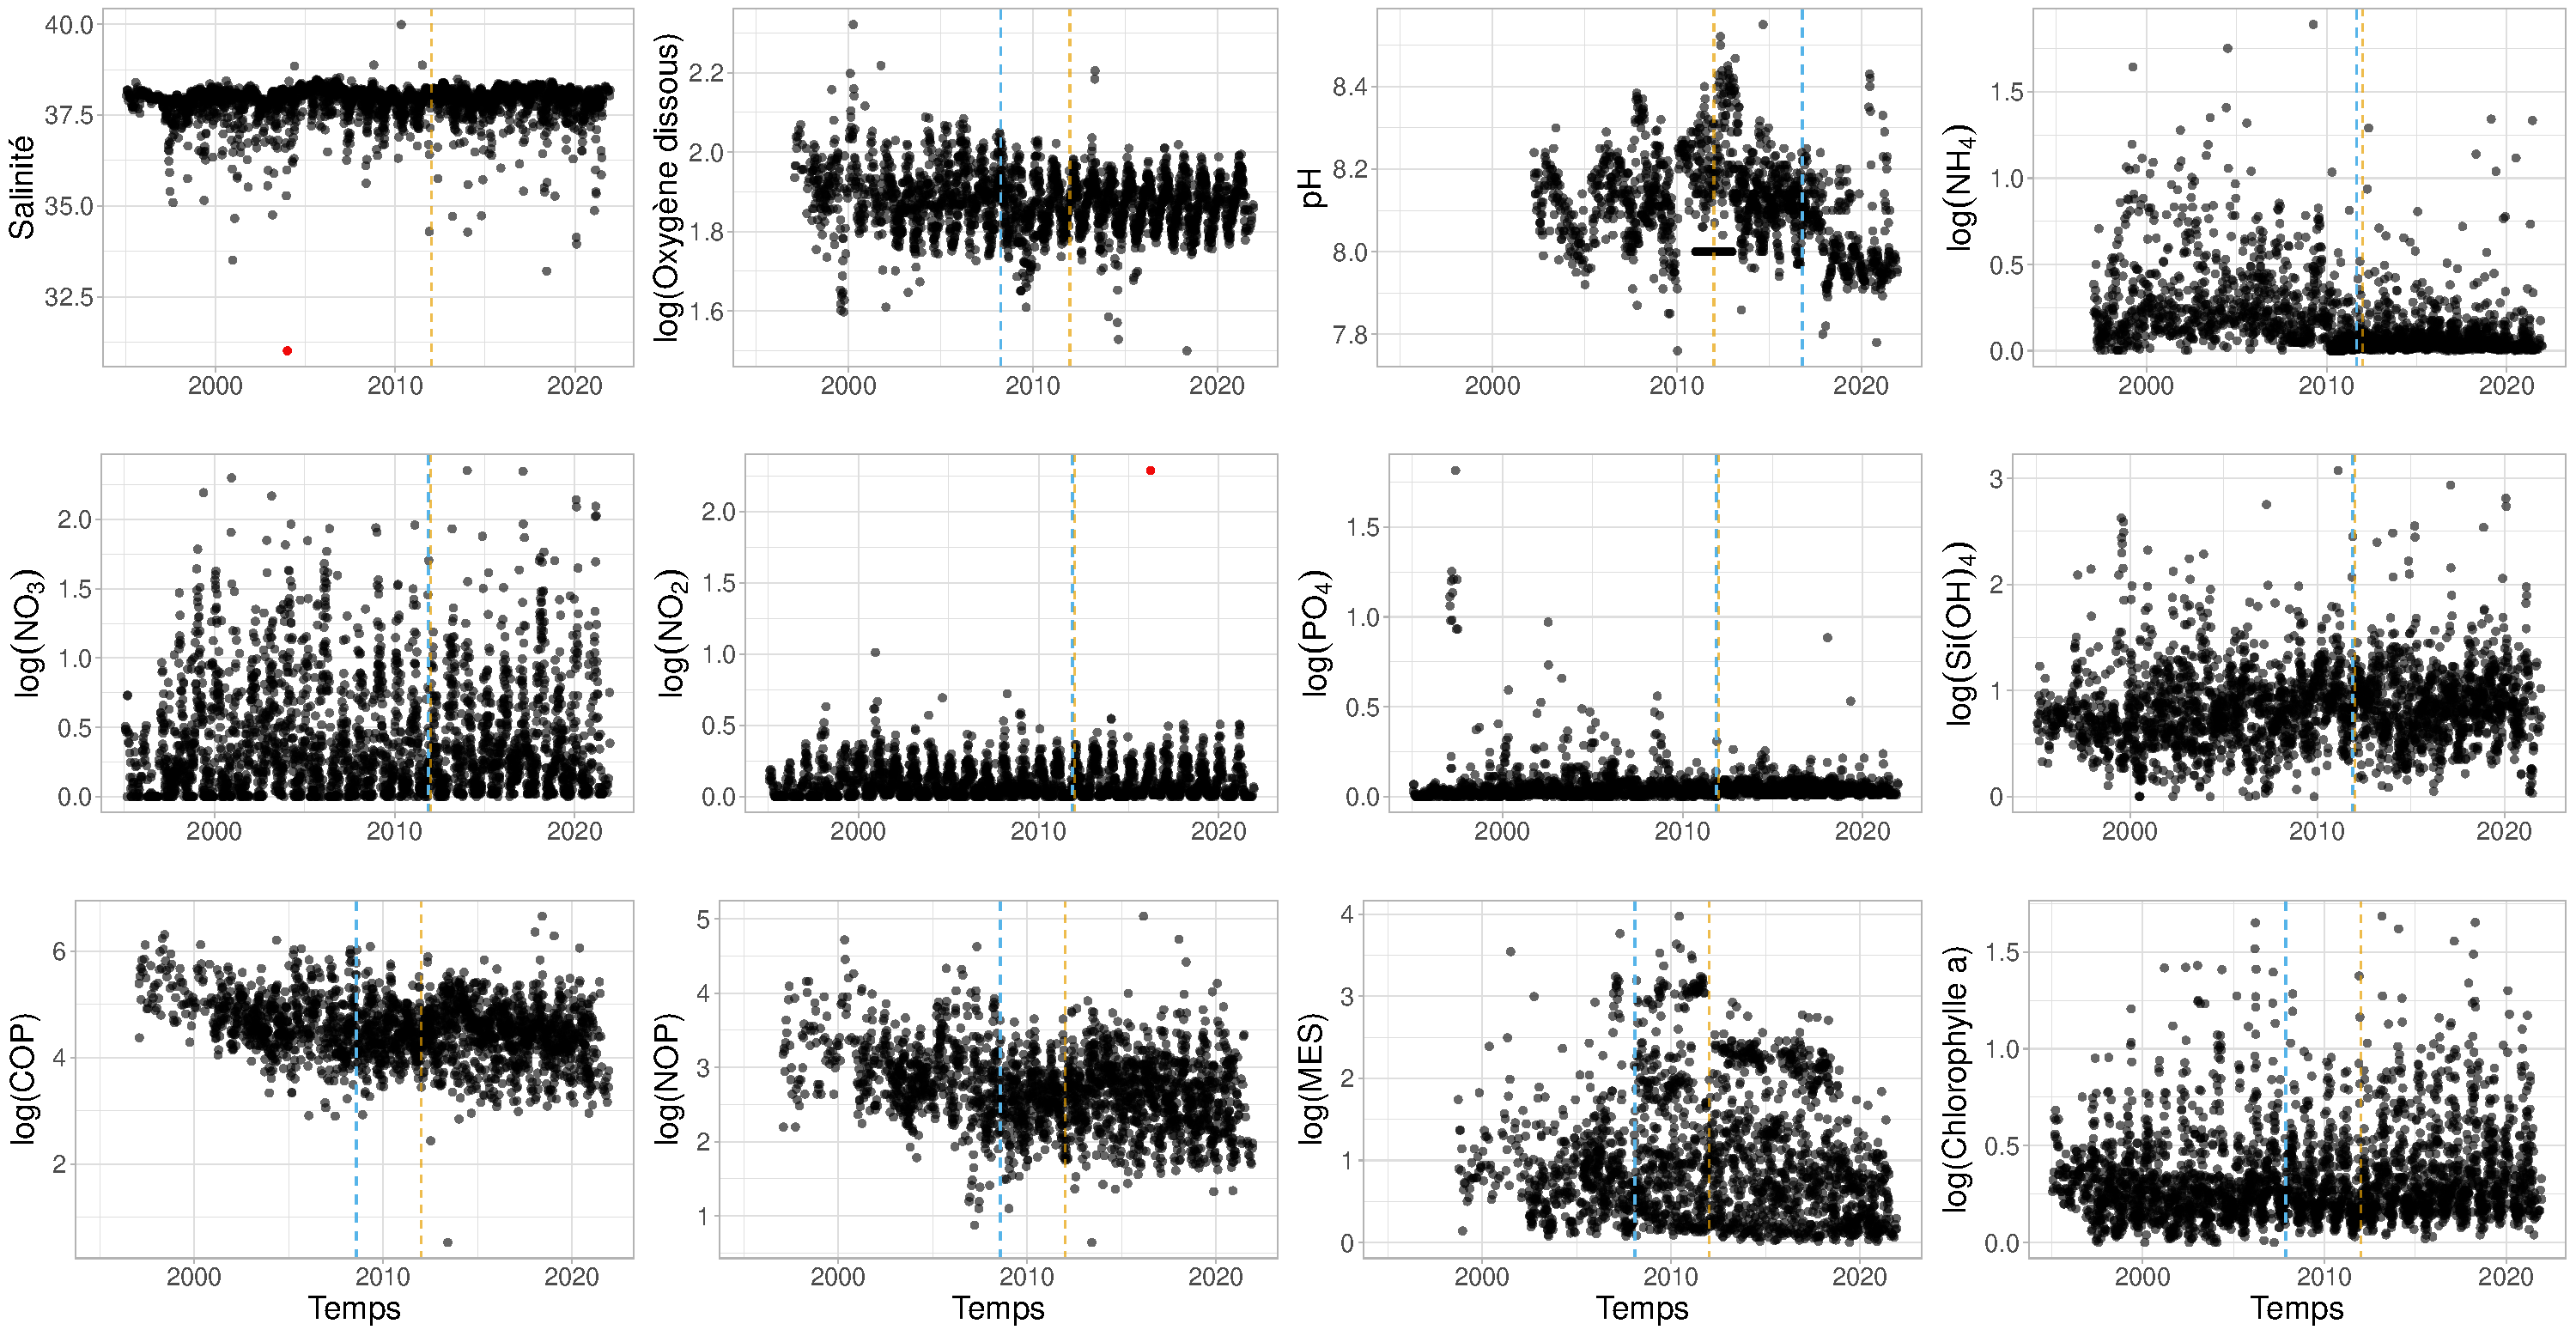
\includegraphics[width=\textwidth]{fig/MM_visualisation_hydro.pdf}
\caption{Séries temporelles des données hydrologiques de surface pour les trois stations SOMLIT méditerranéennes confondues. La ligne pointillé bleue correspond à la mise en place du protocole national pour la variable présentée. La ligne pointillée orange correspond au début du jeu de données PICONANO. Les éventuelles données aberrantes sont représentées en rouge.}
\end{figure}

\begin{figure}
\centering
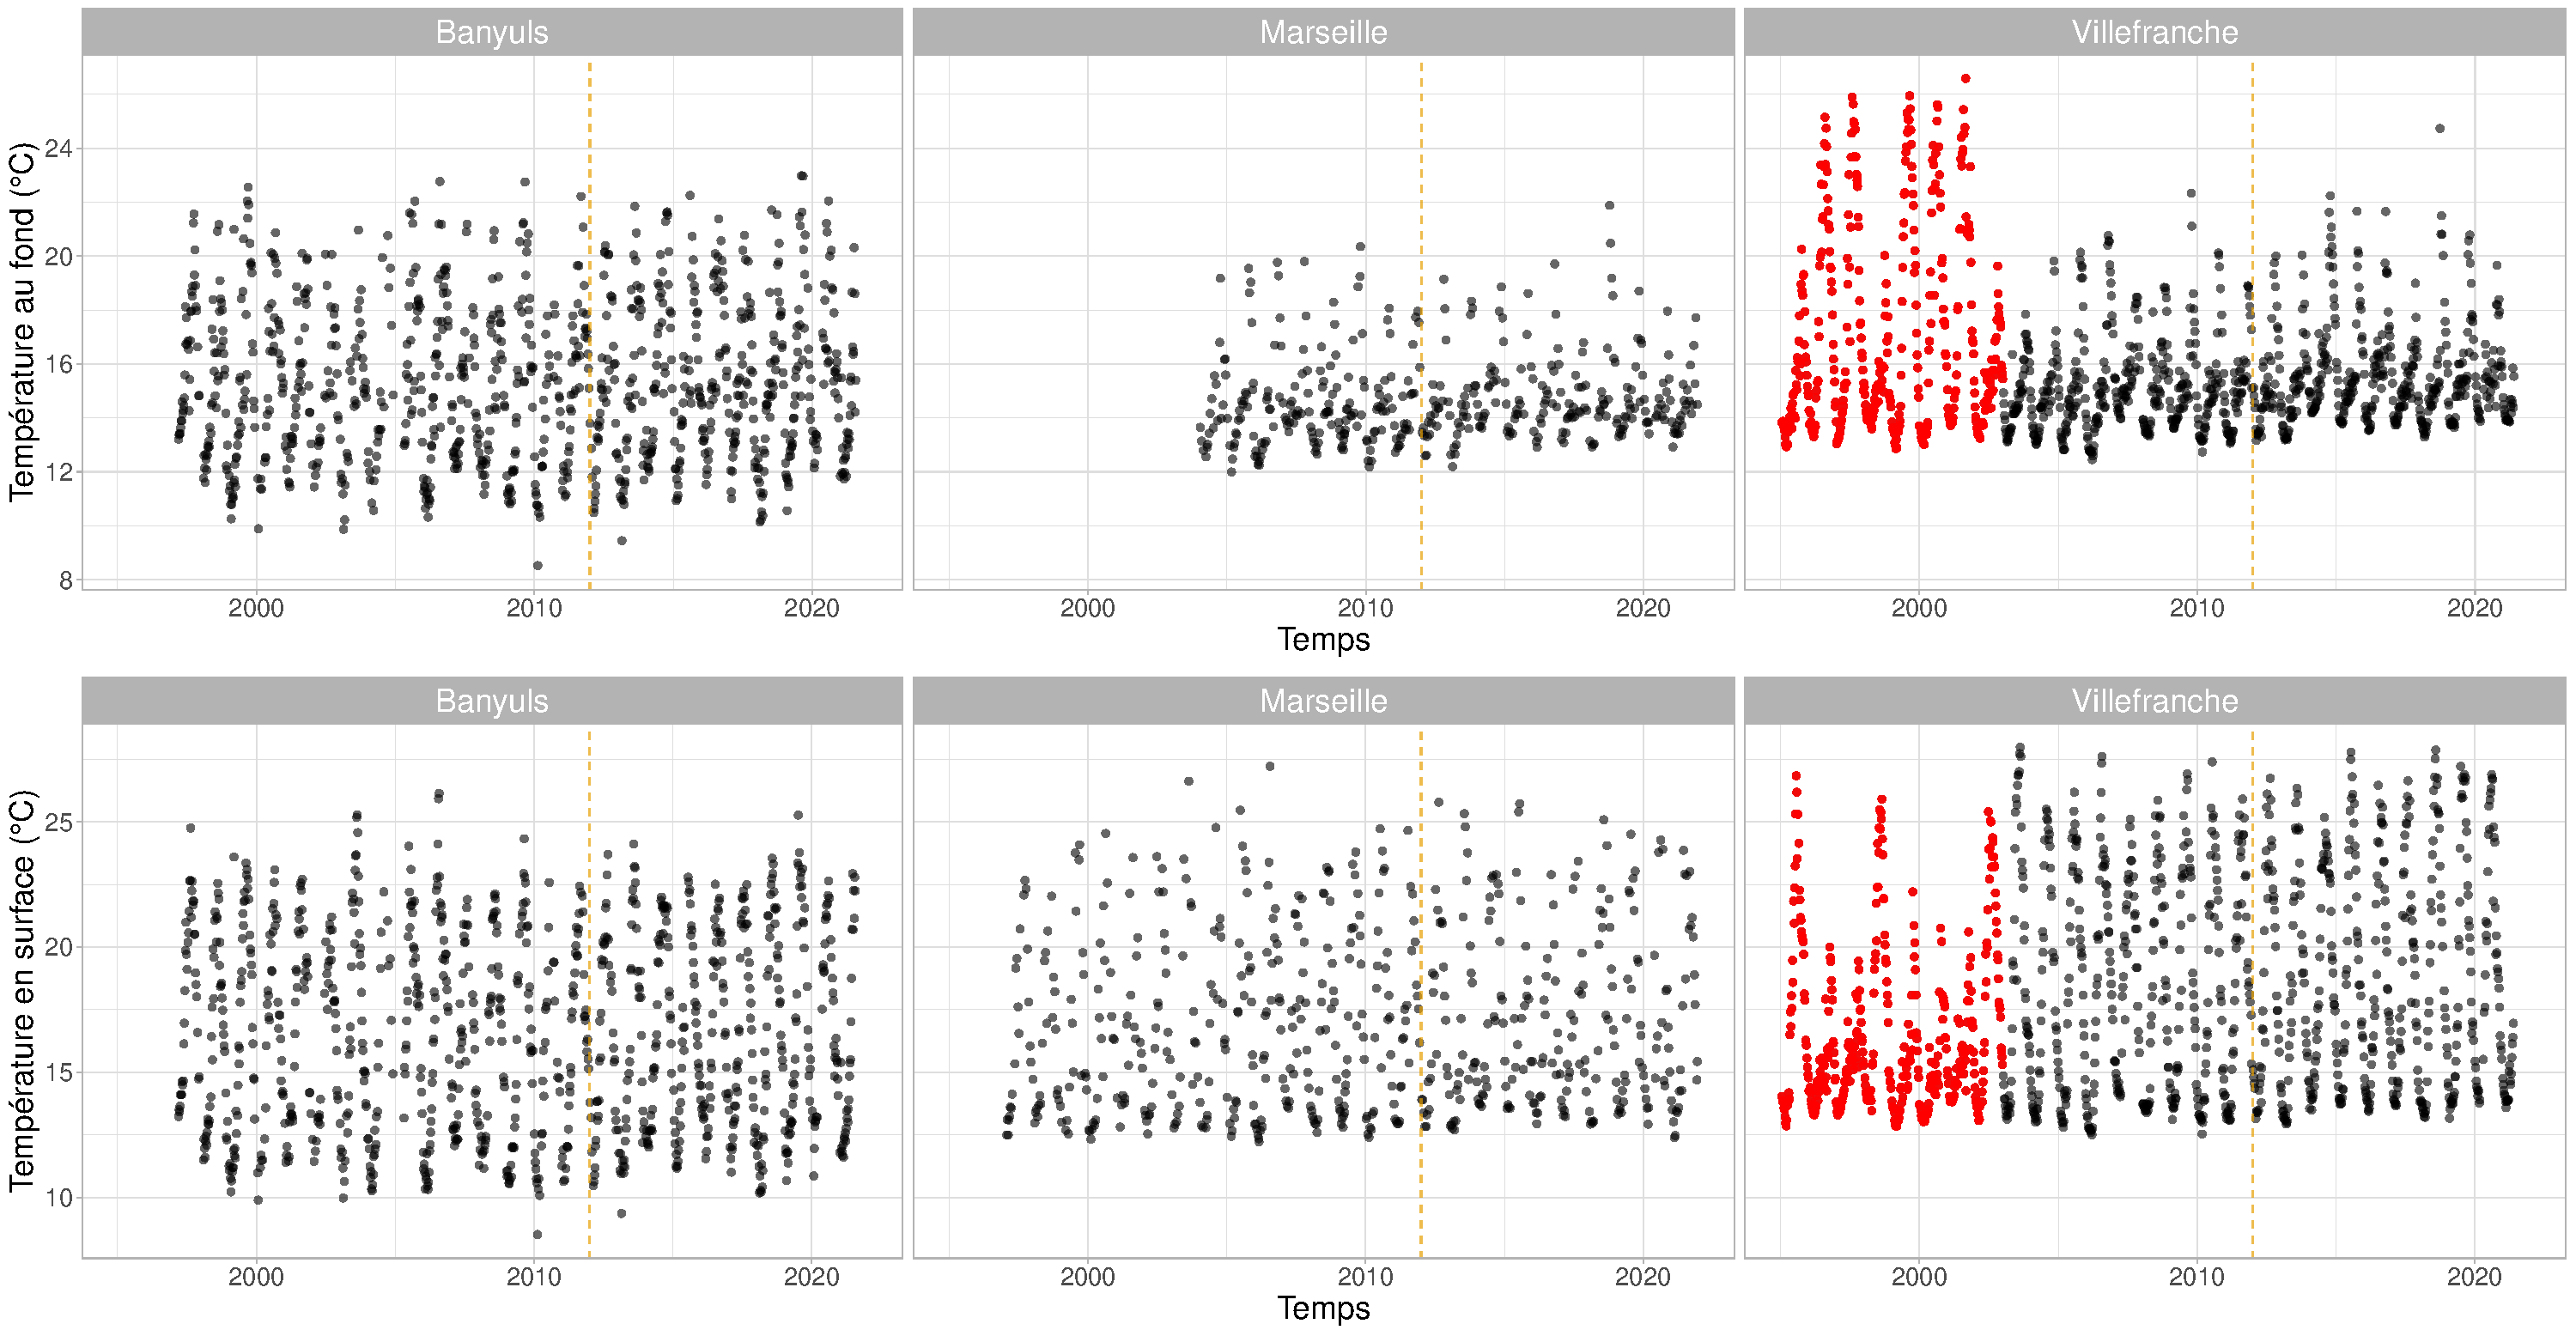
\includegraphics[width=.9\textwidth]{fig/MM_visualisation_T.pdf}
\caption{Séries temporelles des données de Température en surface et au fond pour les trois stations méditerranéennes. La ligne pointillée orange correspond au début du jeu de données PICONANO. Les éventuelles données aberrantes sont représentées en rouge.}
\end{figure}



Dans le cadre de ce stage, seul le phytoplancton est étudié. Par soucis de temps, les bactéries hétérotrophes ne sont pas prises en compte. 
La combinaison des propriétés optiques des cellules, mises en évidence par la cytométrie en flux, permet de distinguer des groupes dans la communauté phytoplanctonique. Si la fluorescence rouge à la chlorophylle présente une gamme étendue de valeur au sein d’une communauté, sa variabilité reste faible au sein d’une même espèce \citet{Trask1982}. Ainsi, la fluorescence à la chlorophylle peut être utilisée pour distinguer des espèces. L’association de la fluorescence rouge à la diffusion lumineuse, indicatrice de la taille et de la structure des cellules, devrait donc permettre d’identifier les groupes fonctionnels décrits précédemment. La Figure 3 représente avec une échelle logarithmique, la valeur moyenne d’auto-fluorescence rouge d’un groupe lors d’un prélèvement, en fonction de la valeur moyenne de diffusion lumineuse.  A l’exception d’une observation pour le groupe des Synechococcus isolée de toutes les autres, les données paraissent fiables puisque l'on identifie facilement les différents groupes. 

\begin{figure}
\centering
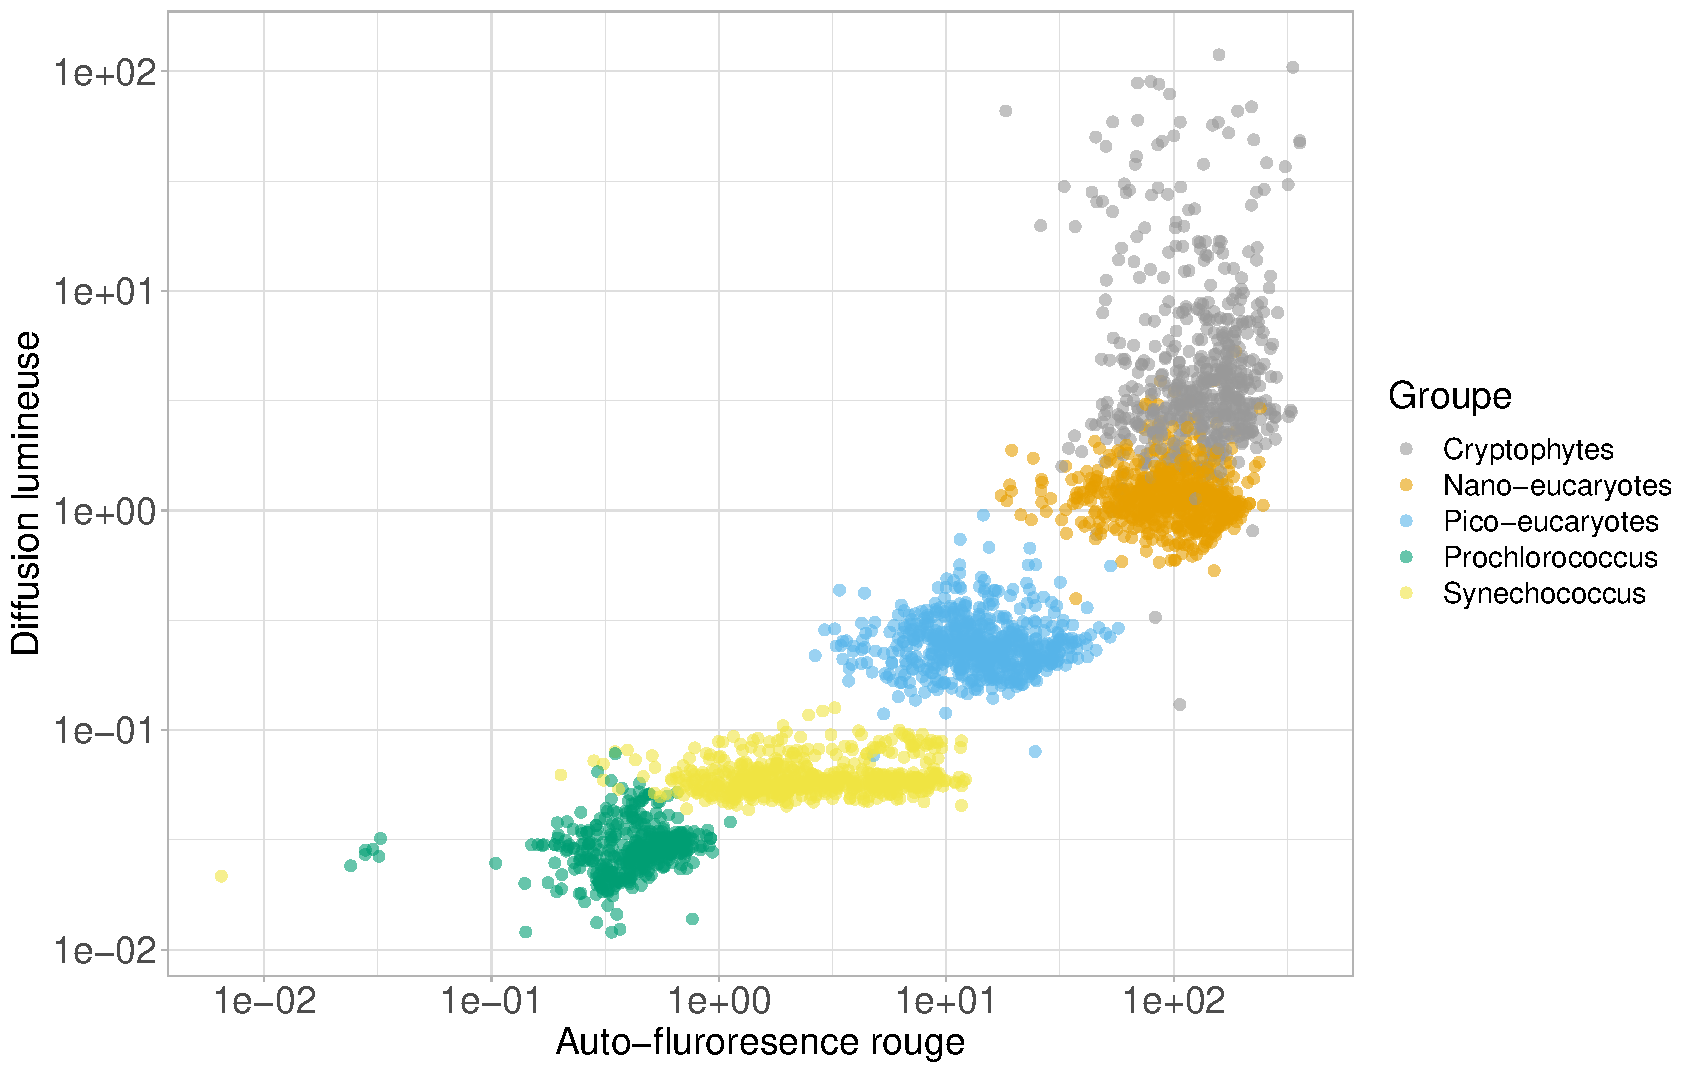
\includegraphics[width=.75\textwidth]{fig/MM_visualisation_phyto.pdf}
\caption{}
\end{figure}


La Figure 4 présente les quatre variables disponibles pour les Synechococcus et les Cryptophytes pour la station de Marseille. Toutes les variables semblent exploitables et pourraient potentiellement apporter des informations pertinentes. Néanmoins, durant ce stage l’étude sera focalisée sur les variables d’Abondance et de Diffusion lumineuse, cette dernière étant indicatrice de la taille moyenne des organismes. 


\begin{figure}
\centering
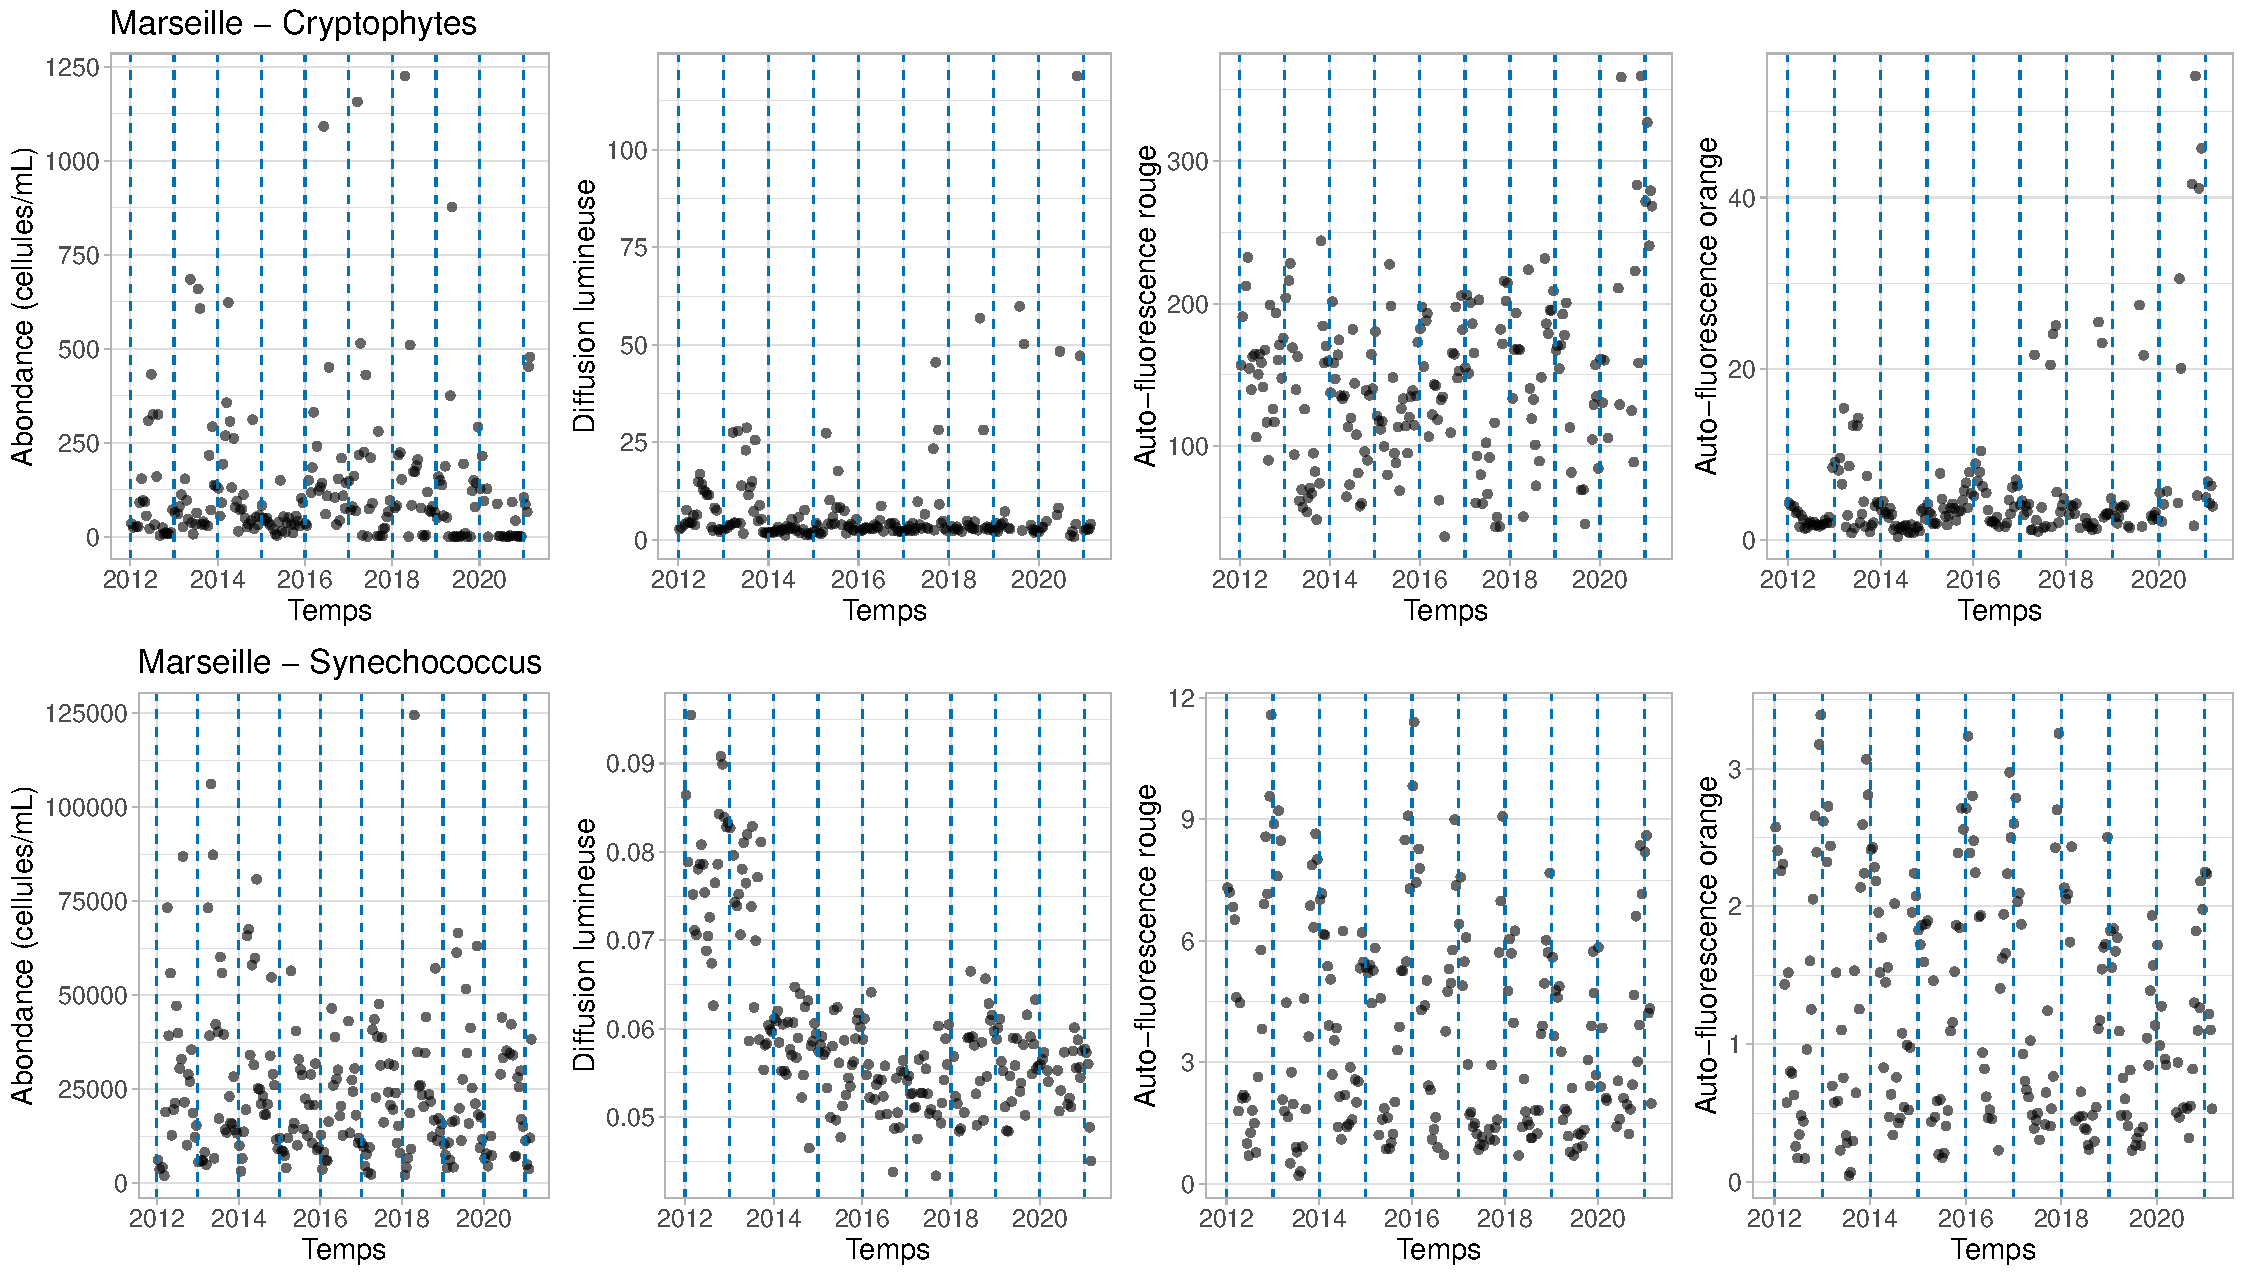
\includegraphics[width=\textwidth]{fig/MM_visualisation_ts_phyto.pdf}
\caption{Série temporelle des données de cytométrie après transformation logarithmique pour les Cryptophytes et Synechococcus pour la station de Marseille. Les lignes pointillées oranges correspondent au 1er janvier de chaque année.}
\end{figure}



\section{Résultats}



\section{Discussion}



\section{Conclusion}


\addcontentsline{toc}{section}{Bibliographie}
\bibliography{biblio.bib}

\newpage
\addcontentsline{toc}{section}{Liste des Figures}
\listoffigures

\addcontentsline{toc}{section}{Liste des Tableaux}
\listoftables

\newpage
\begin{appendices}

\end{appendices}


\begin{abstract}

\end{abstract}

\end{document}
